\section{Afzonderlijke rotatieproef voor G en H}\label{app:gh-rotation}
Deze proef test uitsluitend het toevoegen van $180^\circ$ camera-$y$-rotaties aan G/H-trainingsvoorbeelden. Zij gebruikt geen spiegeltraining, webcamkalibratie of extra voorspelregel. Beide armen blijven gewone 26-letter-SVM's met dezelfde bronbeelden, folds, oorspronkelijke preprocessing, numerieke gamma en klassegewichten.

De draaiing verandert de 210 paar-richtingen volgens $(d_x,d_y,d_z)\mapsto(-d_x,d_y,-d_z)$. Dit is een echte rotatie met determinant $+1$, anders dan horizontale spiegeling. Genormaliseerde afstanden en intrinsieke gewrichtsmetingen blijven gelijk. De bewerking is equivalent aan een polsgerichte draaiing van de beeldhandpunten, maar genereert geen RGB-aanzicht, verborgen vingers of nieuwe detectorfouten.

De historische populatie telt 60.251 geaccepteerde bronnen, waaronder 2.430 G en 2.371 H. Iedere G/H-bron levert het origineel en één draaiing, gewogen met elk 0,5; andere bronnen behouden gewicht één. De volledige trainingsfit heeft 65.052 rijen. De oorspronkelijke toetsbeelden worden niet gedraaid. Een opnieuw getrainde referentie reproduceert alle historische out-of-fold voorspellingen exact.

\begin{table}[h]\centering\small
\caption{Gepoolde resultaten op dezelfde 60.251 ongewijzigde toetsbeelden. P is macro-precisie over A--Z. De percentages zijn conditioneel op succesvolle historische handdetectie.}
\begin{tabular}{lrrrr}\toprule
Training & Acc. (\%) & P (\%) & Macro-F1 & Correct\\\midrule
\tableinput appendix_gh_summary_nl.tex
\bottomrule\end{tabular}\end{table}

Er worden vier fouten hersteld en vijf goede voorspellingen verloren: netto $-1$. De vijf folds hebben respectievelijk netto $+2$, $0$, $-1$, $-1$ en $-1$. Dit geeft geen algemene verbetering op de oorspronkelijke presentatie. Dezelfde toetsfamilie was al bij eerdere ontwikkeling betrokken; dit is geen bevestigende significantieclaim.

\begin{table}[h]\centering\small
\caption{G/H-scores binnen de volledige 26-lettertaak; false positives uit andere letters tellen mee. Dit zijn geen scores van een binaire G/H-classifier.}
\begin{tabular}{llrrrr}\toprule
Letter & Training & N & Precisie & Recall & F1\\\midrule
\tableinput appendix_gh_letters_nl.tex
\bottomrule\end{tabular}\end{table}

G en H hebben dezelfde recall, maar iets lagere precisie en F1 na rotatie. Een gebrek aan winst op deze bronbeelden bewijst niet hoe het model op een nieuwe handrugverzameling zou presteren; zo'n onafhankelijke verzameling ontbreekt. De hier gebruikte hoek en as zijn gekozen na eerdere verkennende proeven, niet op een onaangeroerde eindtest.

\clearpage
\subsection{Datasetbeelden en bekende camerafouten}
De bovenste rij toont twee gelabelde datasetvoorbeelden, de overige rijen vier eerder opgeslagen G/H-gevallen. In de figuur verwijzen [2] en [9] naar de modelknoppen van de applicatie: de wereldgewrichtreferentie en de afzonderlijke rotatievariant. De camerabeelden zijn geen trainingsdata voor deze twee modellen. Zij zijn wel eerder bekeken en in andere kalibratieproeven hergebruikt; hun replay is daarom ontwikkeldiagnostiek.

\begin{figure}[h]\centering
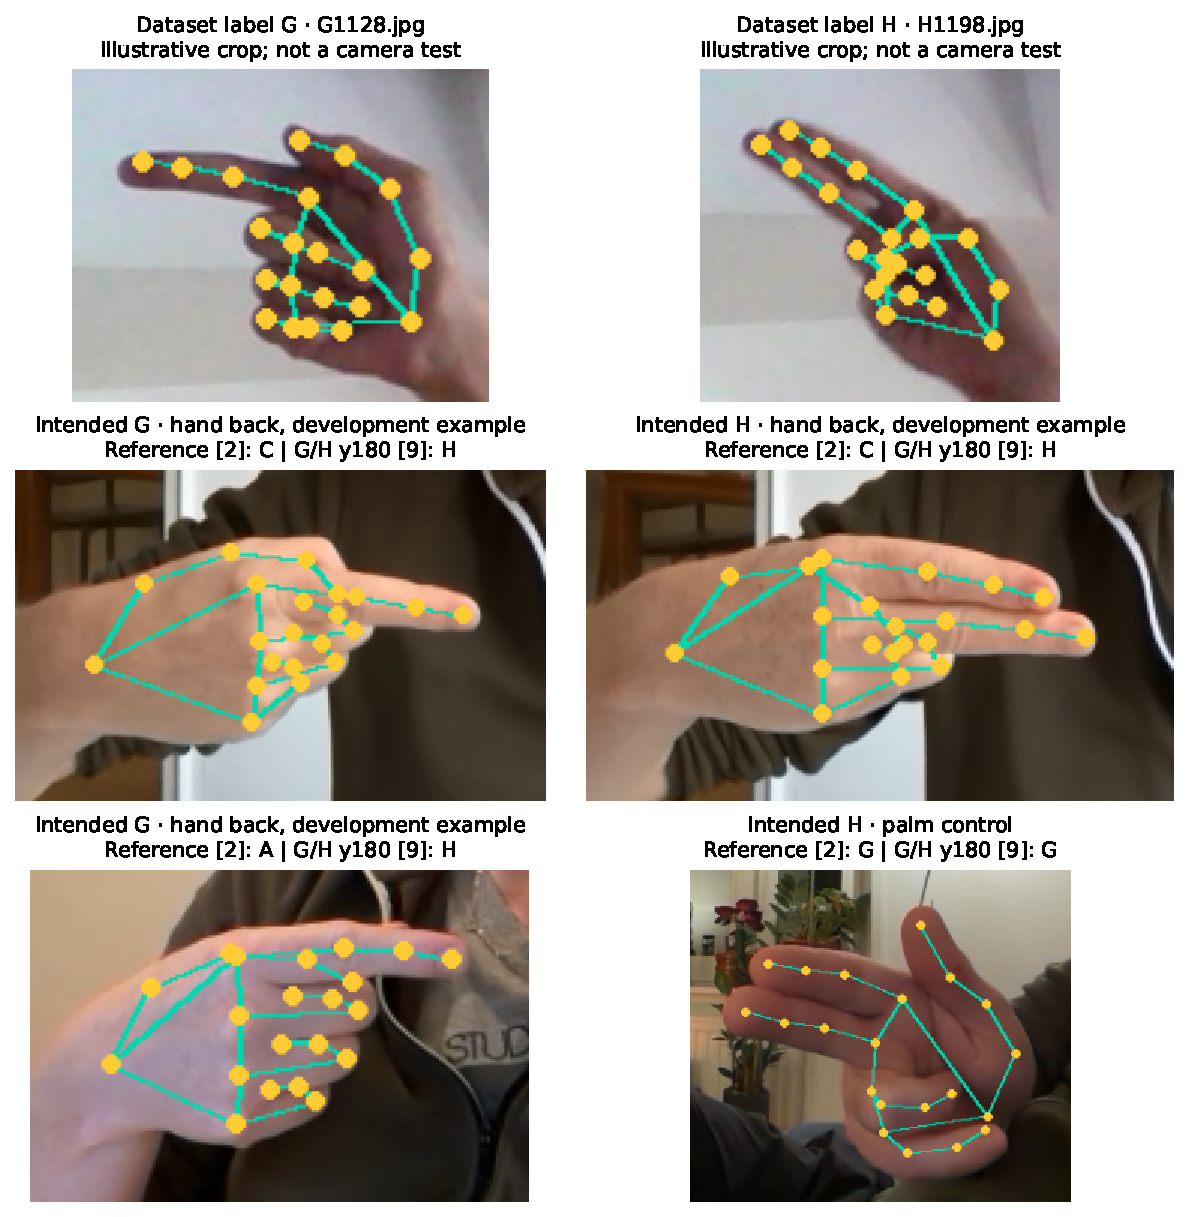
\includegraphics[width=.87\linewidth]{figures/gh_webcam_examples.pdf}
\caption{Uitsneden met de opgeslagen handpunten. Rotatie herstelt de bekende handrug-H, maar beide handrug-G's blijven fout. De palmgerichte H wordt door beide modellen G genoemd. Datasetlabels en kwalitatieve palm-/handrugbeschrijvingen zijn niet onafhankelijk gevalideerd. Aanzicht alleen is hiermee niet aangetoond als oorzaak van alle fouten.}
\end{figure}

De volledige voorspellingen, foldresultaten en verificatie staan in \texttt{results/rotation\_GH\_y180\_01/}. De bron-ID's, beeldhashes en uitsneden staan in \texttt{results/appendix\_visuals\_01/}. Deze controle ondersteunt reproduceerbaarheid van de berekeningen, geen anatomische of nieuwe-persoonsvalidatie.
